\documentclass[tikz,border=4pt]{standalone}
\usepackage{pgfplots}\pgfplotsset{compat=1.18}
\begin{document}
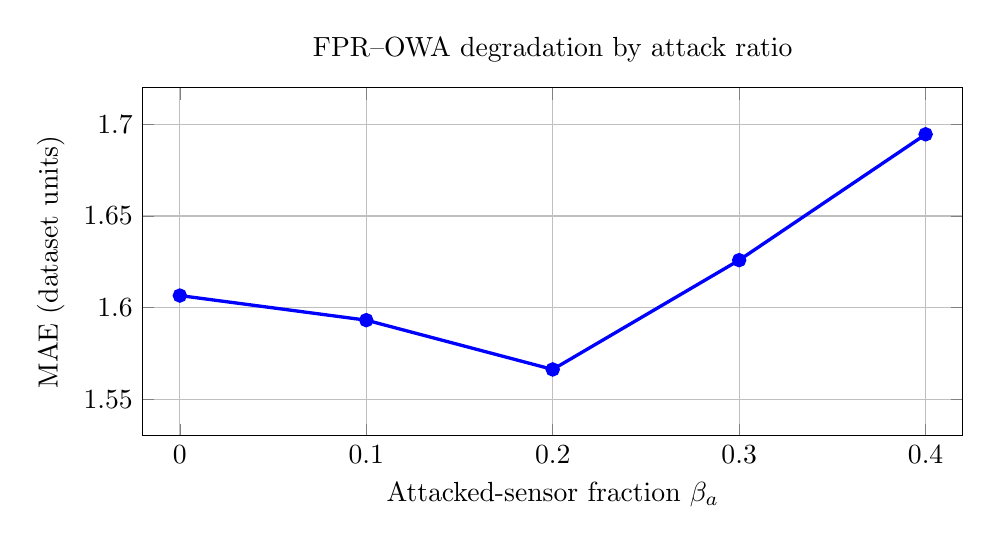
\begin{tikzpicture}
\begin{axis}[width=12cm,height=6cm,xlabel={Attacked-sensor fraction $\beta_a$},
 ylabel={MAE (dataset units)},xmin=-0.02,xmax=0.42,ymin=1.53,ymax=1.72,
 xtick={0,0.1,0.2,0.3,0.4},title={FPR--OWA degradation by attack ratio},grid=major]
\addplot[blue,very thick,mark=*] coordinates {(0,1.606579) (0.1,1.593141) (0.2,1.566224) (0.3,1.625917) (0.4,1.694644)};
\end{axis}\end{tikzpicture}
\end{document}
